\documentclass{beamer}
\usepackage{ctex, hyperref}
\usepackage[T1]{fontenc}

% other packages
\usepackage{latexsym,amsmath,xcolor,multicol,booktabs,calligra}
\usepackage{graphicx,pstricks,listings,stackengine}
\usepackage[normalem]{ulem}

\author{userElaina}
\title{面向人工智能研究的计算机技能分享}
% \subtitle{The Missing Semester of Your CS Education}
\institute{人工智能学院}
\date{2023.12.7}
\usepackage{JilinUniv}

% defs
\def\cmd#1{\texttt{\color{red}\footnotesize $\backslash$#1}}
\def\env#1{\texttt{\color{blue}\footnotesize #1}}
\definecolor{deepblue}{rgb}{0,0,0.5}
\definecolor{deepred}{rgb}{0.6,0,0}
\definecolor{deepgreen}{rgb}{0,0.5,0}
\definecolor{halfgray}{gray}{0.55}

\lstset{
    basicstyle=\ttfamily\small,
    keywordstyle=\bfseries\color{deepblue},
    emphstyle=\ttfamily\color{deepred},    % Custom highlighting style
    stringstyle=\color{deepgreen},
    numbers=left,
    numberstyle=\small\color{halfgray},
    rulesepcolor=\color{red!20!green!20!blue!20},
    frame=shadowbox,
}

\begin{document}

\kaishu
\begin{frame}
    \titlepage
    \begin{figure}[htpb]
        \begin{center}
            
\includegraphics[width=0.15\linewidth]{pic/Jilin_University_Logo.eps}
        \end{center}
    \end{figure}
\end{frame}

\begin{frame}
\tableofcontents[sectionstyle=show,subsectionstyle=show/shaded/hide,subsubsectionstyle=show/shaded/hide]
\end{frame}

% cs dalao: 写个教案

% \section{背景}

% \begin{frame}{由来及参考}
%     \begin{itemize}
%         \item MIT: The Missing Semester of Your CS Education (计算机教育中缺失的一课)
%         \item ZJU-竺院: 实用技能拾遗
%         \item "很长时间你们都被困在墙内" % miss 的比 ZJU 还要多一点
%     \end{itemize}
% \end{frame}

% zju: 绪论,shell + cli (+ vim), git(hub), latex, 文档排版, docker

\section{Environment}

\begin{frame}{mirrors}
    \begin{itemize}
        \item Tuna, BFSU, HIT, USTC, ..., JLU!
        \item pip install \_ -i https://mirrors.jlu.edu.cn/pypi/simple/
        \item /etc/apt/source.list
        \item /etc/pacman.d/mirrorlist
        \item pacman-mirrors
    \end{itemize}
\end{frame}

\begin{frame}{mirrors}
    \begin{figure}[c]
        \centering
        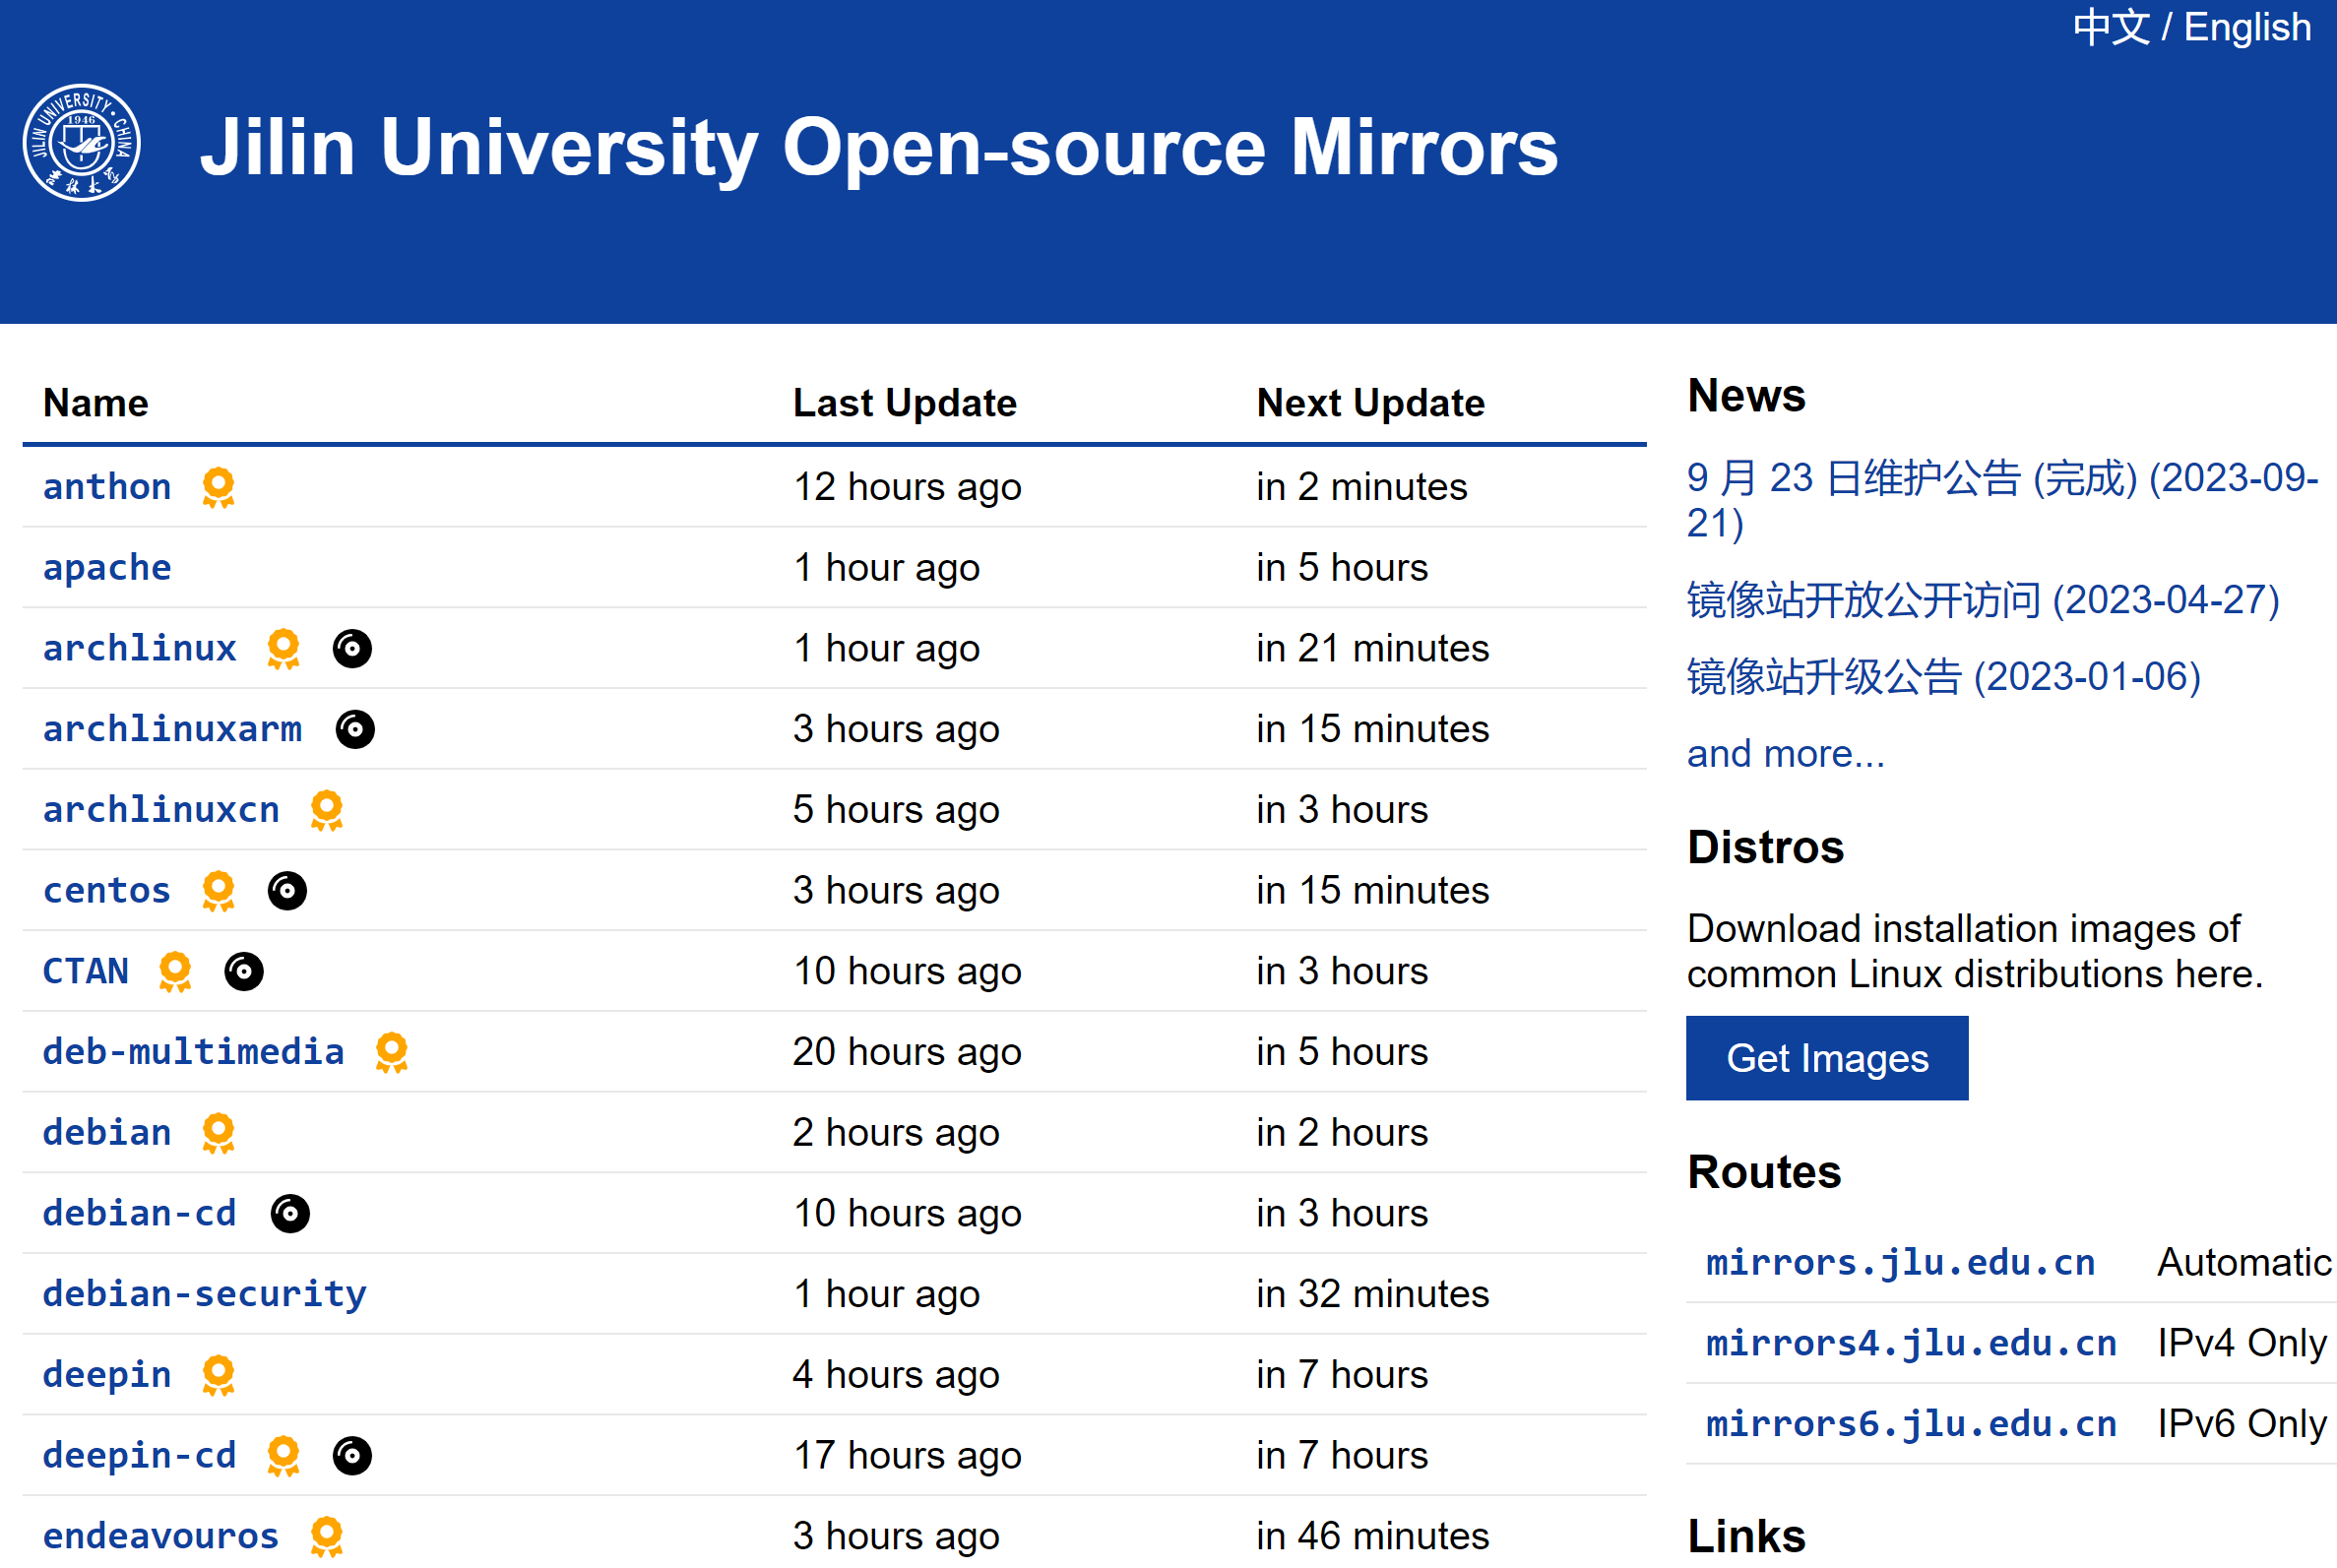
\includegraphics[height=.8\textheight]{pic/mirror.png}
        \caption{https://mirrors.jlu.edu.cn/}
    \end{figure}
\end{frame}

\begin{frame}{mirrors}
    \begin{figure}[c]
        \centering
        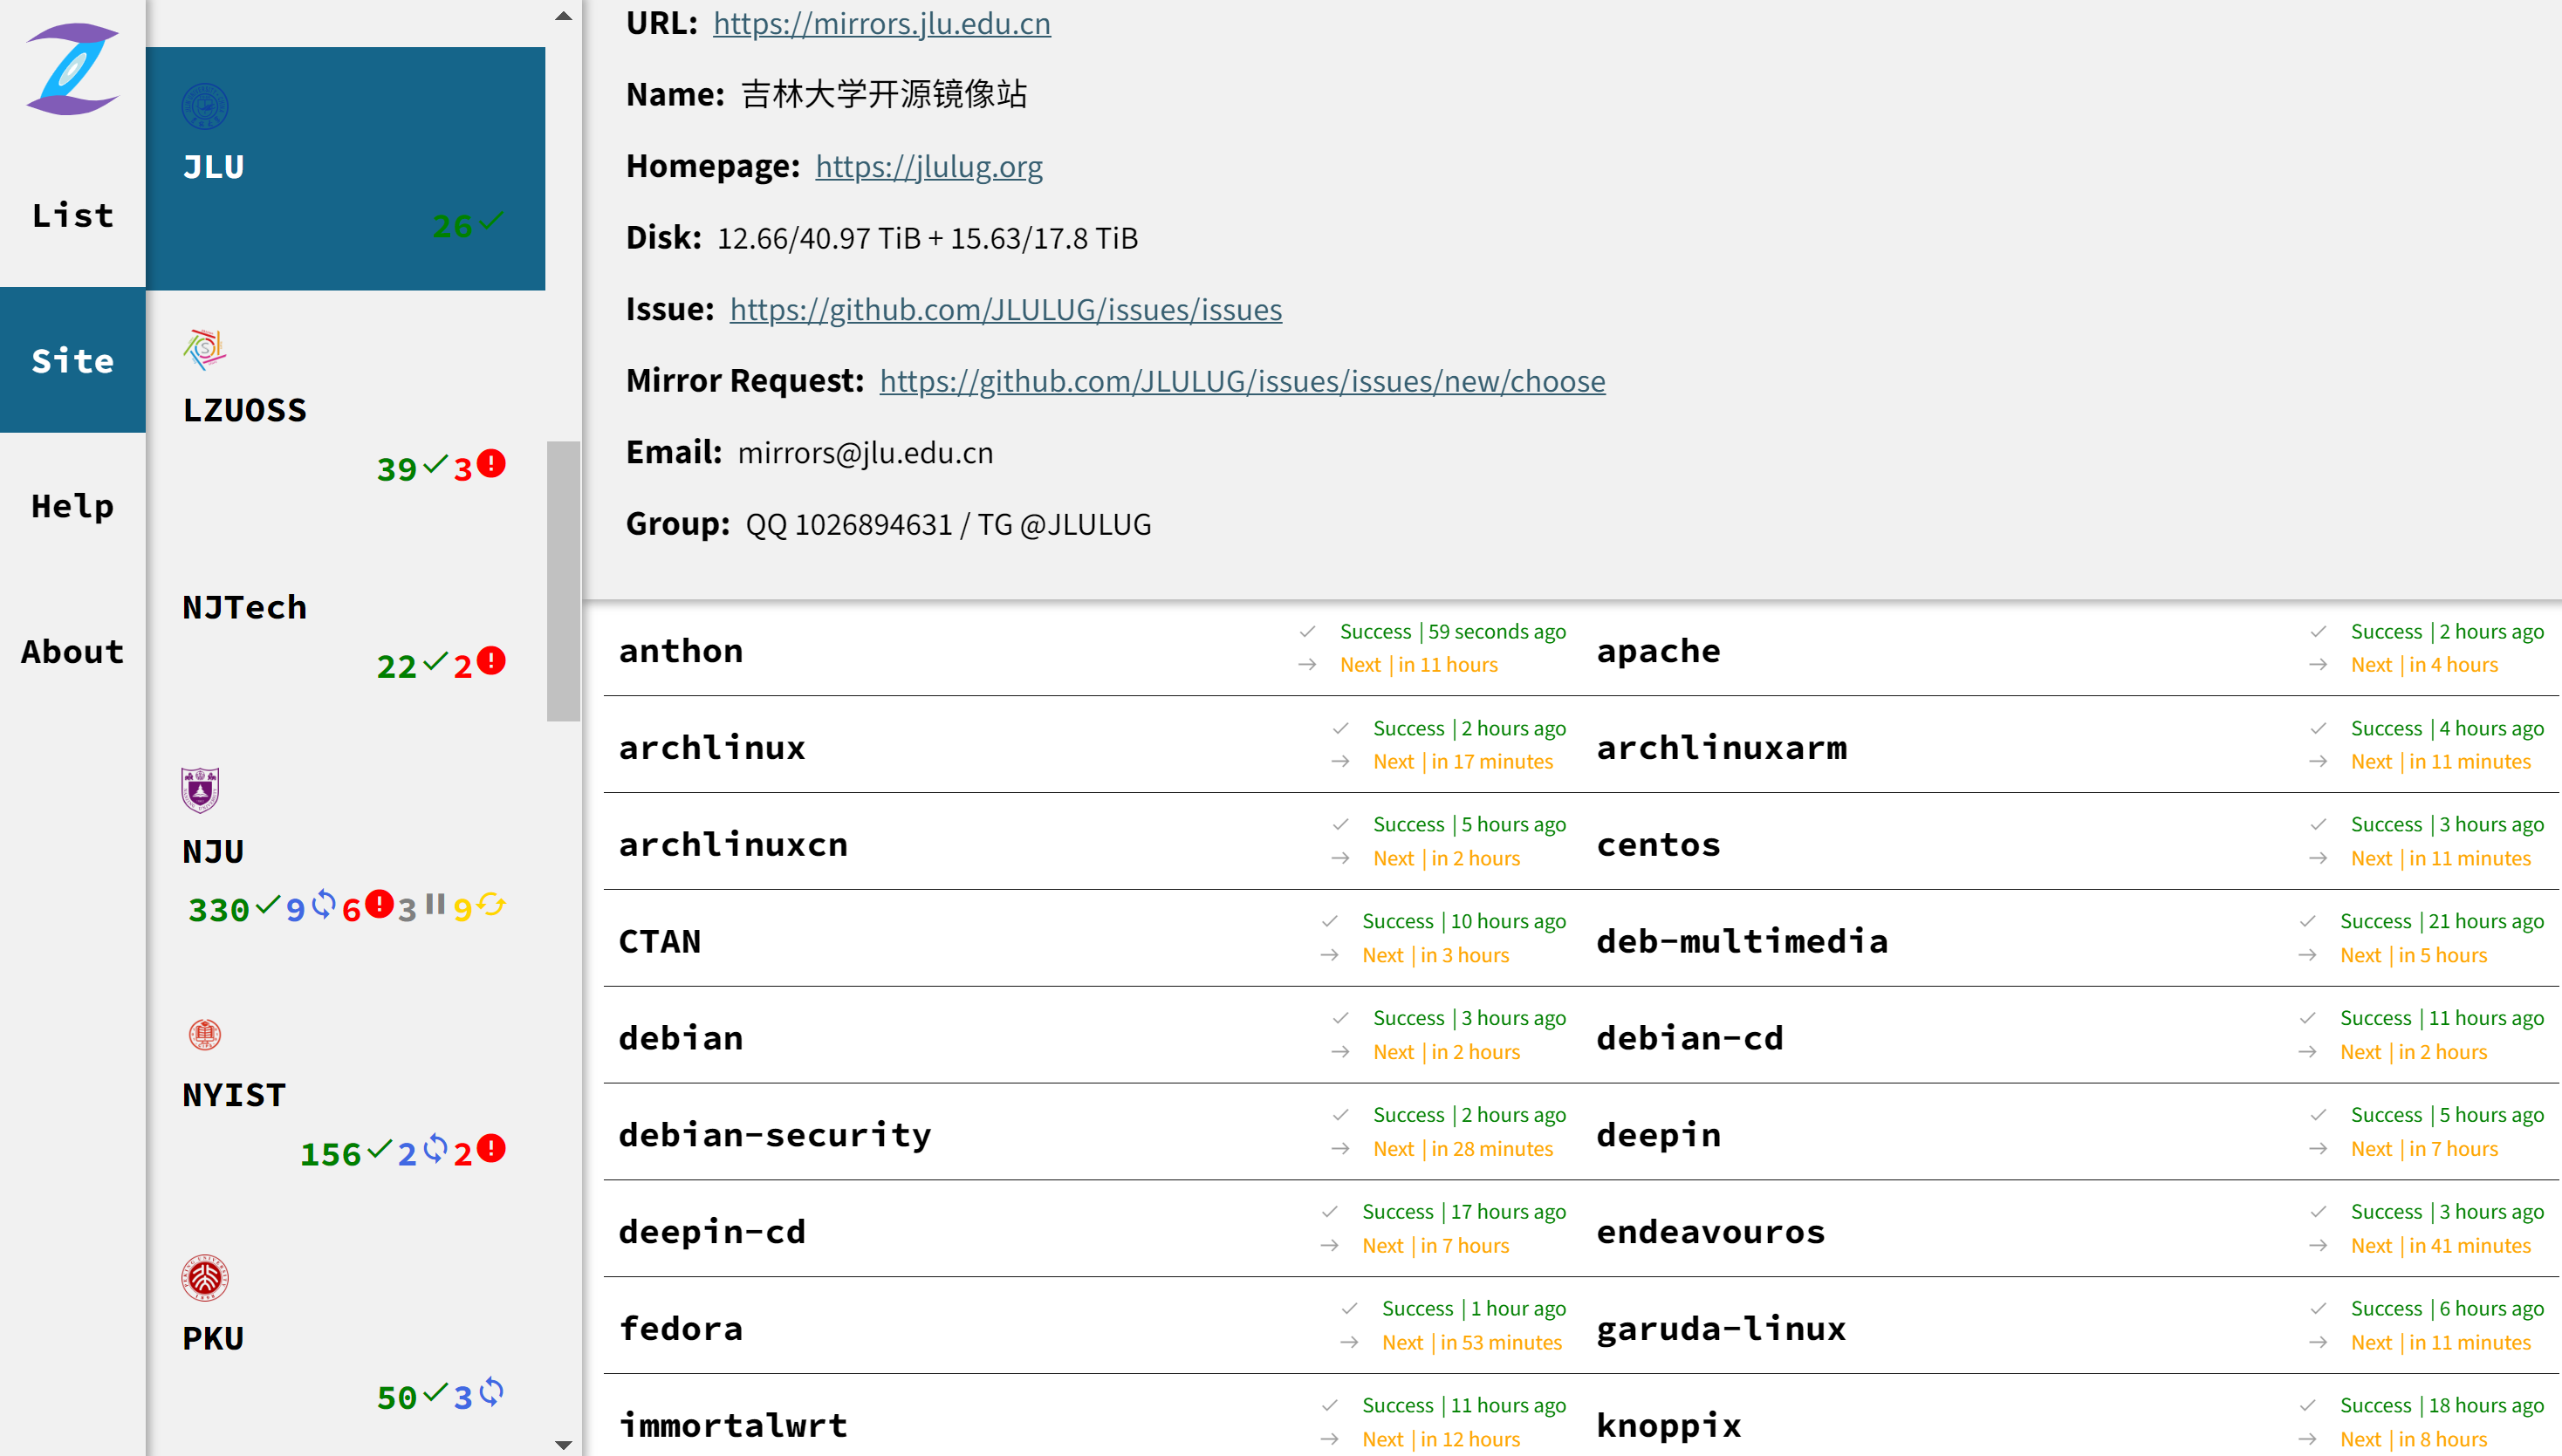
\includegraphics[height=.7\textheight]{pic/mirrorz.png}
        \caption{MirrorZ.org}
    \end{figure}
\end{frame}

\begin{frame}{proxy}
    \begin{itemize}
        \item WebVPN 助手: https://greasyfork.org/scripts/395271
        \item 包管理器使用代理: https://github.com/rosebe/FUCK-GFW
        \item Transparent Proxy
    \end{itemize}
\end{frame}

\begin{frame}{proxy}
    \begin{itemize}
        \item \begin{figure}[c]
            \centering
            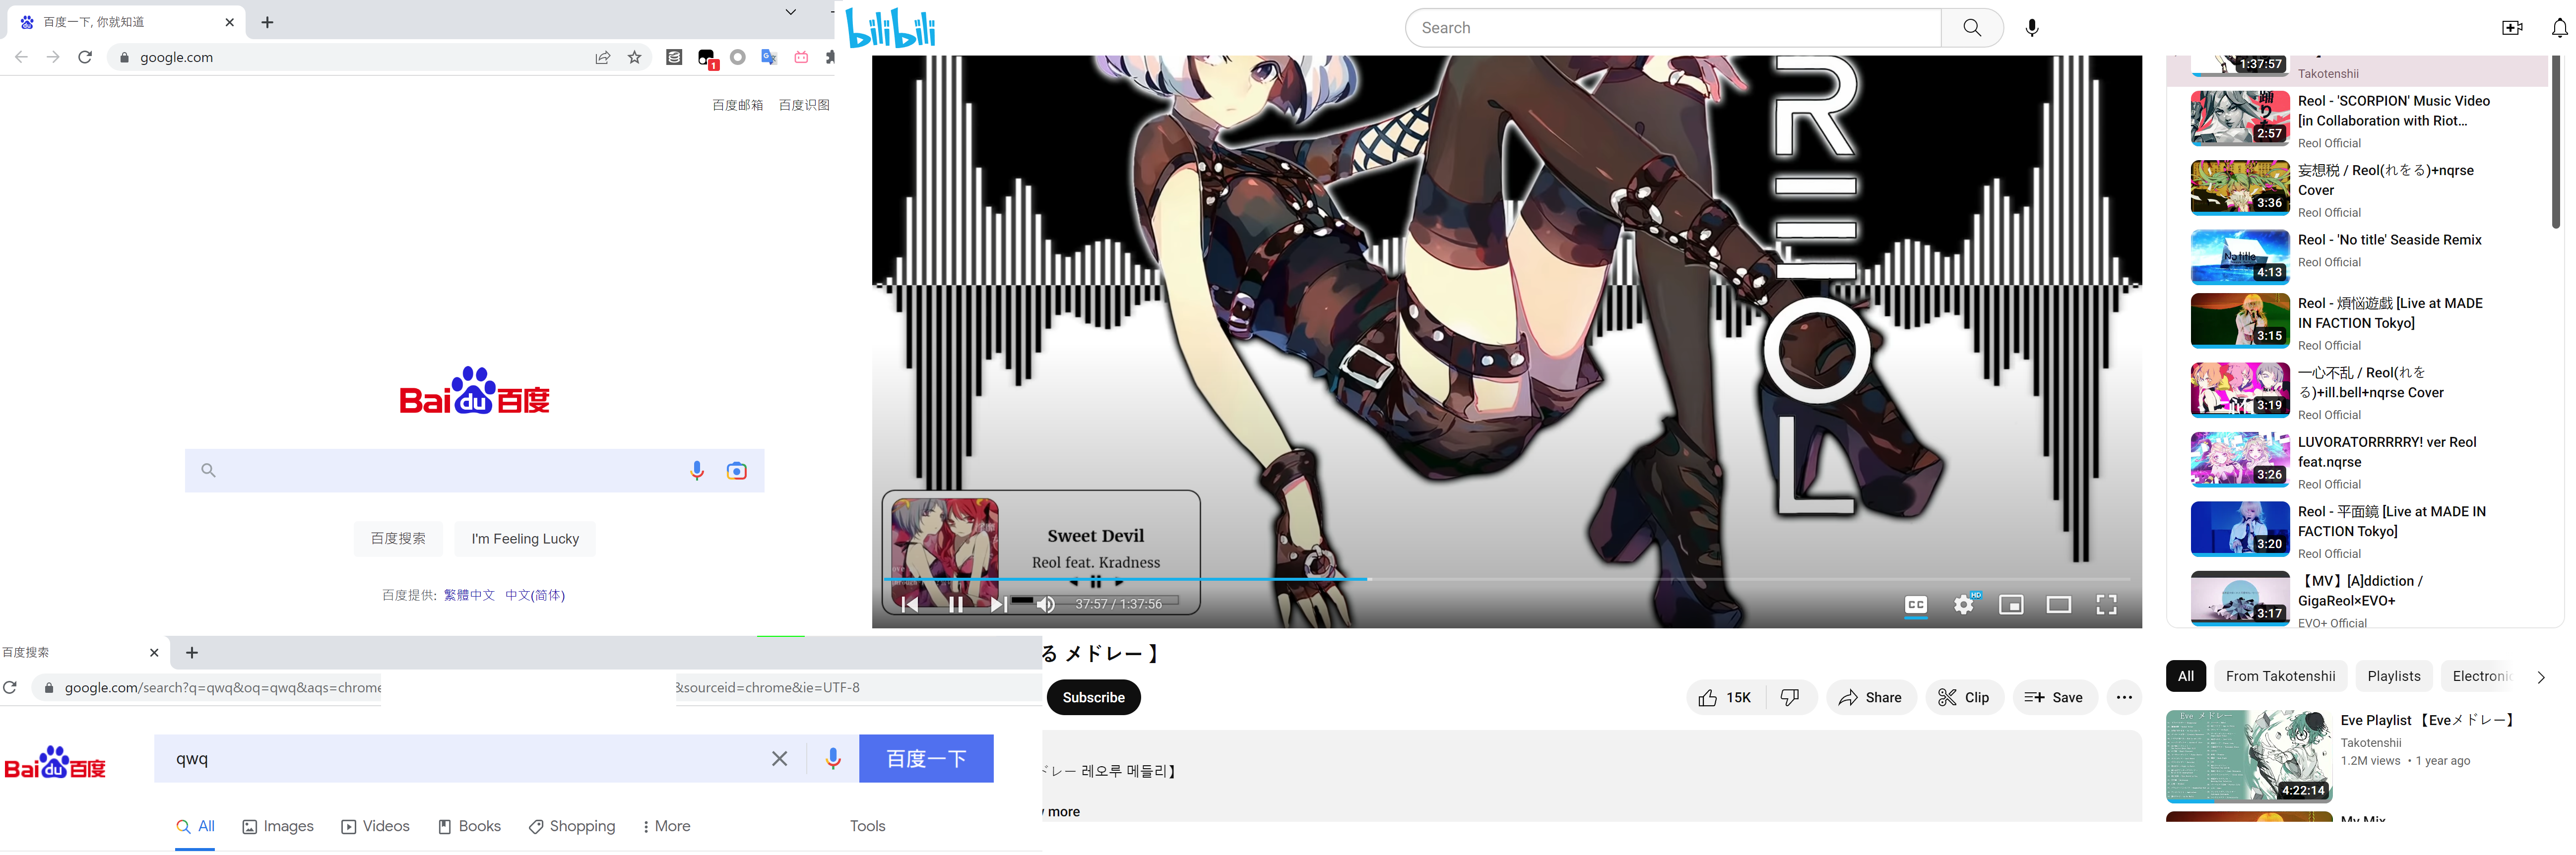
\includegraphics[height=.5\textheight]{pic/gf.png}
            \caption{将国际网站伪装成中国网站}
        \end{figure}
        \item https://github.com/userElaina/this-is-the-China-website
        \item https://greasyfork.org/scripts/461427
    \end{itemize}
\end{frame}

\begin{frame}{虚拟环境}
    \begin{itemize}
        \item py -m venv ENV\_DIR
        \item Anaconda
        \item Docker
        \item VM (WSL, Sandbox, Hyper-V, VMware, Qemu...)
    \end{itemize}
\end{frame}

\section{Linux}

\begin{frame}{shell}
    \begin{itemize}
        \item bash, zsh, fish
        \item man, --help
        \item Vim
        \item cat, find, diff, grep, awk
        \item Git, GitHub
        \item make, cmake
        \item ssh -p 50022 user@nas.mil
        \item scp -P 50022 -r ./localfolder/ user@192.168.1.2:/mnt/t1/
    \end{itemize}
\end{frame}

\begin{frame}{后台运行}
    \begin{itemize}
        \item \sout{\&}
        \item nohup CMD > LOG 2>\&1 \&
        \item screen
        \item Tmux
    \end{itemize}
\end{frame}

\begin{frame}{Distribution}
    \begin{itemize}
        \item Debian and Ubuntu
        \item Arch Linux and Manjaro
        \item RHEL and CentOS
        \item Kali Linux and Black Arch Linux
        \item Deepin
    \end{itemize}
\end{frame}

% \section{硬件}

% \begin{frame}{硬件加速}
%     \begin{itemize}
%     \end{itemize}
% \end{frame}

% \begin{frame}{硬件选购}
%     \begin{itemize}
%     \end{itemize}
% \end{frame}

\section{杂项}

% \begin{frame}{Markdown}
%     \begin{itemize}
%     \end{itemize}
% \end{frame}

\begin{frame}{LaTeX}
    \begin{itemize}
        \item Template
        \item Overleaf
        \item IEEE
    \end{itemize}
\end{frame}

\section{致谢}

\begin{frame}{由来及参考}
    \begin{itemize}
        \item MIT: The Missing Semester of Your CS Education (计算机教育中缺失的一课)
        \item ZJU-竺院: 实用技能拾遗
        \item "很长时间你们都被困在墙内" % miss 的比 ZJU 还要多一点
    \end{itemize}
\end{frame}

\begin{frame}{Q \& A}
    \begin{center}
        {\Huge\calligra Thanks!}
    \end{center}
\end{frame}

\end{document}
